\section{Сравнение LLM моделей для Text-to-SQL}

В рамках исследования были сопоставлены три модели: \texttt{Qwen/Qwen3-Coder-Next},
\texttt{GLM-4.7} и \texttt{GigaChat-2}. Для оценки использовался набор из 31
SQL-задачи разного уровня сложности, охватывающий типовые сценарии работы с
реляционными данными: \texttt{SELECT DISTINCT}, \texttt{GROUP BY}, \texttt{HAVING},
агрегатные функции, фильтрацию по датам, соединения таблиц, подзапросы, CTE, работу
с JSON-полями, а также более сложные запросы с вычисляемыми показателями и
ограничениями по бизнес-логике. Такой набор позволяет оценить не только способность
модели генерировать синтаксически корректный SQL, но и её устойчивость к задачам,
где требуется точное понимание структуры данных и условий запроса.

Каждая модель тестировалась в двух режимах: \textbf{без самокоррекции} (базовый
режим, в котором модель генерирует ответ за один проход) и \textbf{с
самокоррекцией} (модель получает обратную связь об ошибке выполнения и повторно
генерирует запрос). Такое разделение позволяет оценить как базовые возможности
модели, так и её способность исправлять допущенные ошибки.

По сводным метрикам лучший результат в обоих режимах показала \texttt{GLM-4.7}.
В режиме без самокоррекции её показатели составили: Execution Accuracy (EA) —
54,8\%, Exact Matching Accuracy (EM) — 25,8\%, ESM — 35,5\% и Intellect — 64,5\%.
После включения самокоррекции значения улучшились до 67,7\%, 38,7\%, 48,4\% и 77,4\%
соответственно. \texttt{Qwen} в базовом режиме набрала 45,2\%, 19,4\%, 29,0\% и
54,8\%, а с самокоррекцией — 61,3\%, 32,3\%, 41,9\% и 71,0\%. Наиболее слабые
результаты продемонстрировала \texttt{GigaChat-2}: без самокоррекции — 16,1\%,
6,5\%, 9,7\% и 22,6\%, с самокоррекцией — 29,0\%, 12,9\%, 22,6\% и 38,7\%. Таким
образом, самокоррекция дала прирост всем трём моделям, однако не устранила
принципиального разрыва между ними. Сравнение метрик без режима самокоррекции и после
его включения представлено на рисунках \ref{llm_before} и \ref{llm_after}.

\begin{figure}[H]
    \centering
    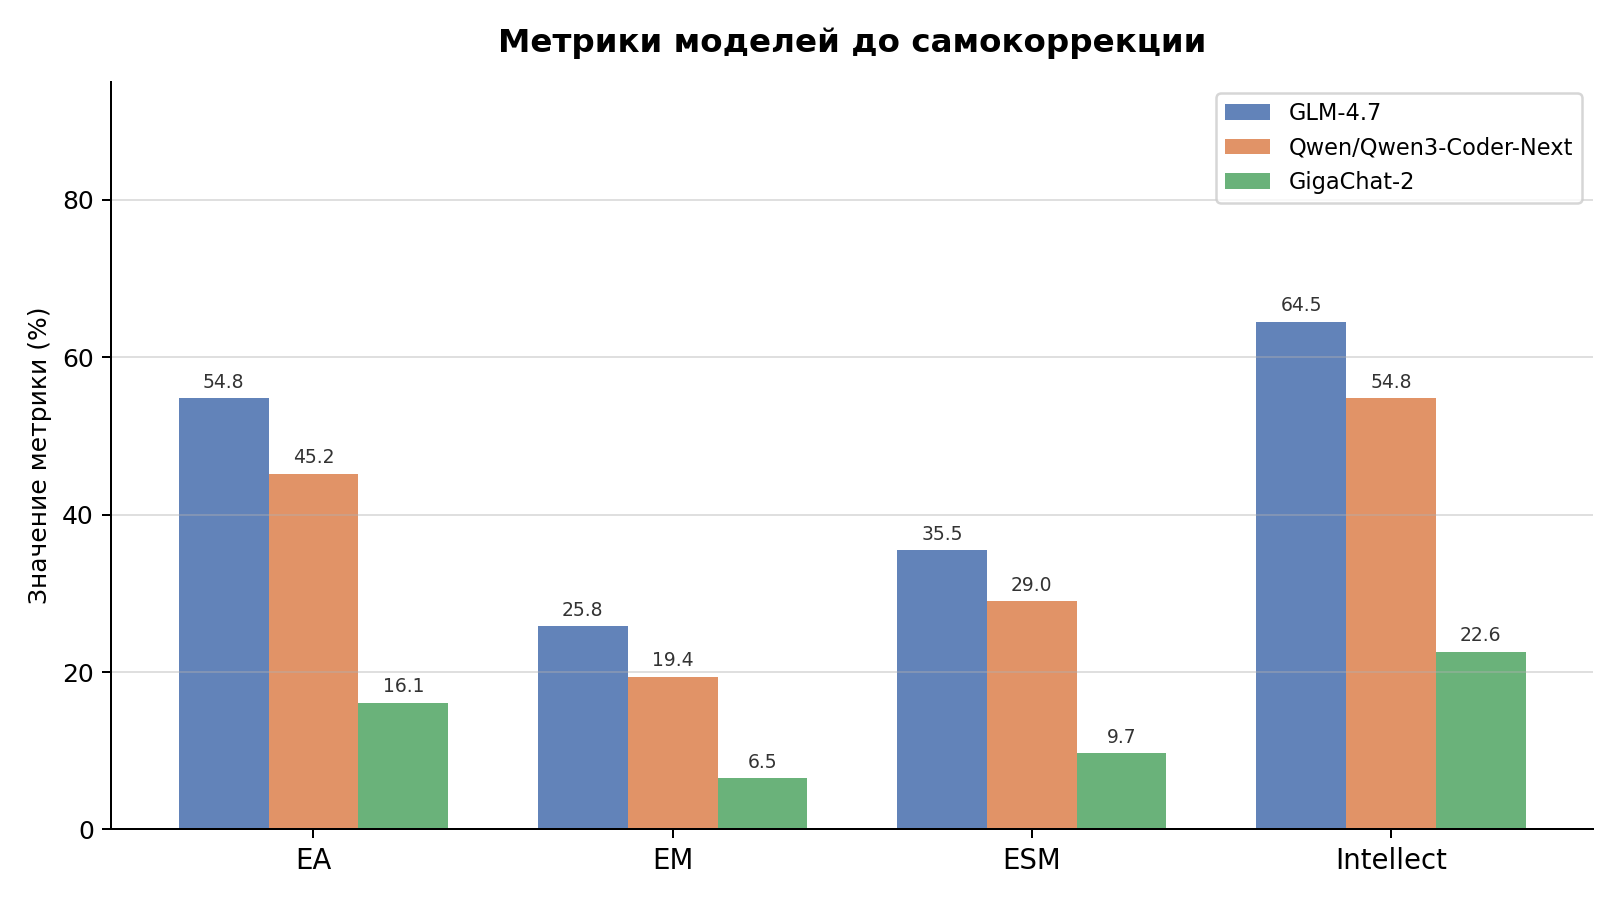
\includegraphics[width=\textwidth]{materials/llm_before.png}
    \caption{Метрики LLM без режима самокоррекции}
    \label{llm_before}
\end{figure}


\begin{figure}[H]
    \centering
    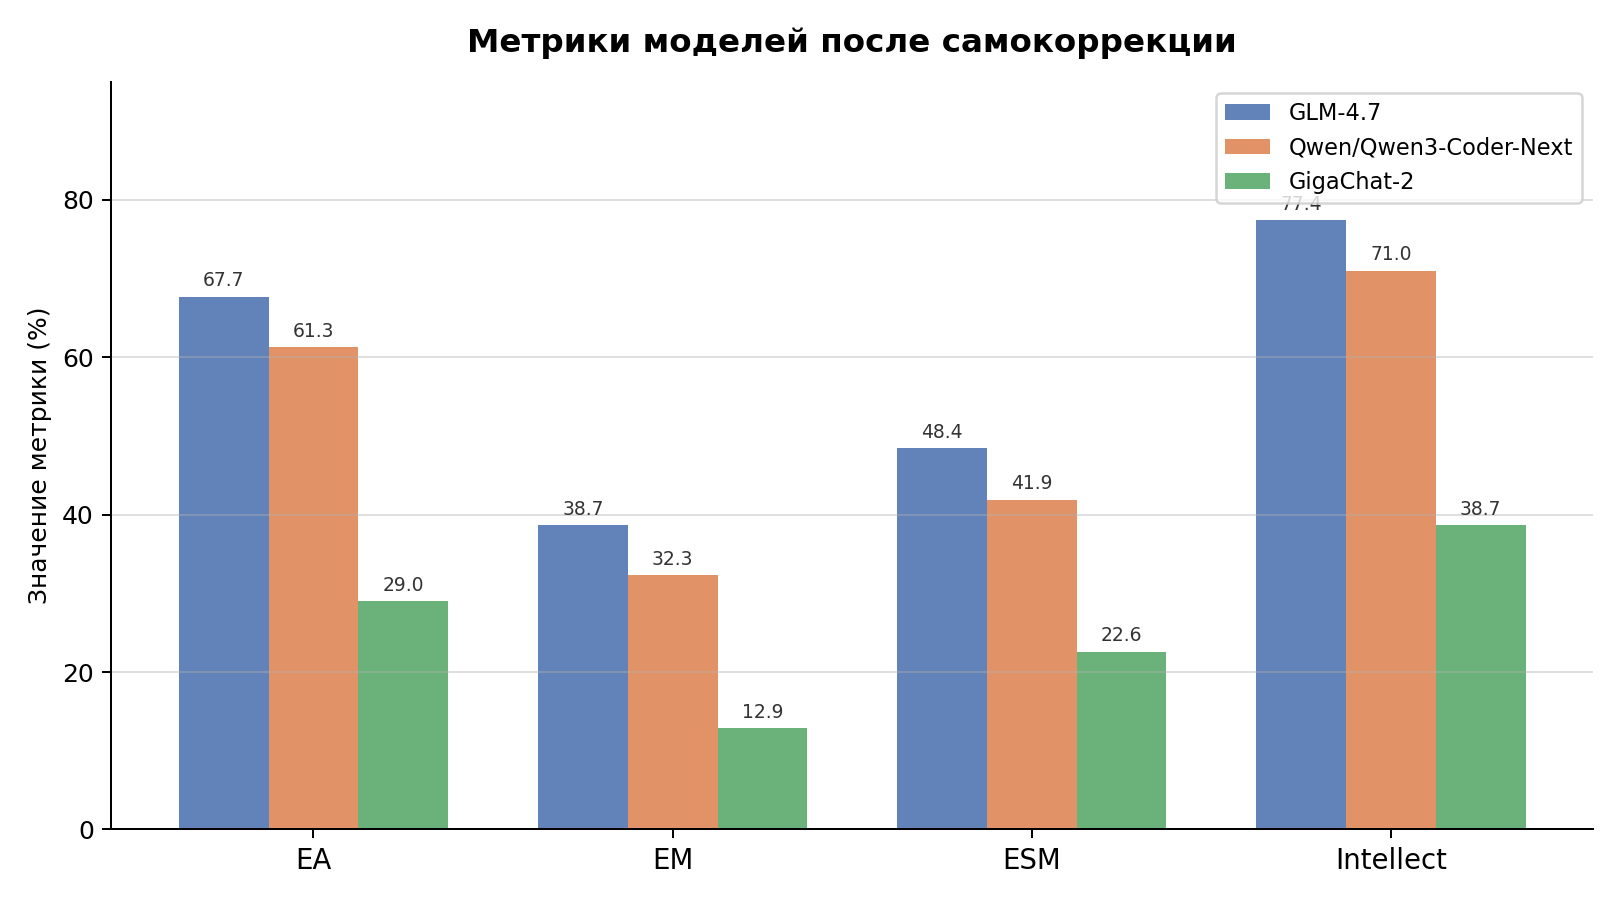
\includegraphics[width=\textwidth]{materials/llm_after.png}
    \caption{Метрики LLM после режима самокоррекции}
    \label{llm_after}
\end{figure}

\subsection{Анализ метрик}

Важно отметить, что между Execution Accuracy и Exact Matching наблюдается заметный
разрыв у всех моделей — как в базовом режиме, так и после самокоррекции. Это
означает, что часть ответов не совпадает с эталоном по форме, но при этом выполняет
задачу корректно. Иными словами, модели нередко предлагали семантически верные, но
синтаксически отличающиеся SQL-запросы: меняли имена столбцов, порядок полей, стиль
записи, использовали альтернативные, но эквивалентные конструкции. В самом
исследовании отдельно отмечено, что более мягкая метрика IEA / Intellect учитывает
именно такие случаи и лучше отражает реальную практическую полезность ответа.
Поэтому при интерпретации результатов важно смотреть не только на точное совпадение
текста SQL, но и на фактическую корректность результата.

\subsection{Влияние режима самокоррекции}

Самокоррекция оказала положительный эффект на все модели, однако степень улучшения
существенно различается. \texttt{GLM-4.7} продемонстрировала прирост EA на 13,0
п.п.\ (с 54,8\% до 67,7\%), \texttt{Qwen} — на 16,1 п.п.\ (с 45,2\% до 61,3\%).
\texttt{GigaChat-2} также улучшила показатели, но в меньшей мере: EA выросла лишь
на 12,9 п.п.\ (с 16,1\% до 29,0\%), а по метрике EM прирост составил всего 6,4
п.п. Это свидетельствует о том, что \texttt{GigaChat} хуже использует возможность
повторной генерации: даже получая сигнал об ошибке, она нередко воспроизводила
исходный некорректный запрос с незначительными изменениями.

\subsection{Сравнение моделей}

\subsubsection{Qwen/Qwen3-Coder-Next}

Модель хорошо проявила себя на простых и средних задачах, где требовались
стандартные операции над таблицами: выбор уникальных значений, группировка, подсчёт
записей и простая фильтрация. Например, она успешно справлялась с задачами про
уникальные коды самолётов, уникальные аэропорты, подсчёт аэропортов по странам,
сортировку пассажиров по алфавиту и несколькими типовыми запросами по бронированиям
и рейсам. Вместе с тем на более сложных задачах \texttt{Qwen} теряла устойчивость:
это видно по заданиям, где требовались вычисляемые показатели, более тонкая работа
с условиями фильтрации, соединения нескольких таблиц или извлечение данных из
JSON-полей. В таких случаях модель могла либо ошибаться в логике запроса, либо не
выдерживать требуемую структуру ответа. Самокоррекция помогала \texttt{Qwen}
исправить часть подобных ошибок, что обеспечило наиболее заметный относительный
прирост среди трёх участников.

\subsubsection{GLM-4.7}

\texttt{GLM-4.7} показала наиболее сбалансированное поведение в обоих режимах.
Сильной стороной модели стала способность корректно решать как базовые, так и более
содержательные запросы: например, задачи с извлечением русскоязычного названия модели
самолёта, подсчётом статистики по рейсам, выборкой аэропортов в России, расчётом
агрегатов по классам обслуживания и вычислением задержек рейсов. Особенно
показательно, что \texttt{GLM} часто давала семантически верный запрос даже тогда,
когда точное текстовое совпадение с эталоном отсутствовало. Режим самокоррекции
позволил модели дополнительно улучшить результаты, преимущественно за счёт задач
средней сложности, где первоначальный запрос содержал незначительные структурные
погрешности. При этом \texttt{GLM} не идеальна: в ряде случаев она тоже ошибалась,
особенно когда требовалось очень строгое соблюдение формата ответа или нетривиальная
логика объединения таблиц.

\subsubsection{GigaChat-2}

\texttt{GigaChat-2} показала самый слабый результат в обоих режимах тестирования.
В базовом режиме для неё характерны частые ошибки в выборе таблиц, путаница в
названиях полей, некорректные соединения и трудности с удержанием нескольких условий
одновременно. На простых задачах модель иногда справлялась — например, при выборе
уникальных значений, базовых подсчётах или простых фильтрах. Однако по мере
усложнения задания качество резко падало. Особенно заметны проблемы на запросах с
CTE, подзапросами, вычисляемыми метриками, датами, сложной агрегацией и связями
между несколькими сущностями. Самокоррекция дала лишь ограниченный эффект:
\texttt{GigaChat} нередко повторяла исходные ошибки или вносила изменения, не
устранявшие суть проблемы. В некоторых кейсах модель фактически не могла выдать
рабочий запрос даже после нескольких итераций. Это говорит о слабой устойчивости
модели к прикладным SQL-задачам средней и высокой сложности и об ограниченной
способности к самодиагностике ошибок.

\subsection{Сложные запросы}

Отдельно стоит отметить, что существуют задания, с которыми не справились все три
модели ни в одном из режимов. К таким случаям относятся наиболее сложные запросы,
где требовалось совместить несколько логических операций: сложные соединения,
ограничения по дате, вычисления по выборке и строгую структуру результат. Подобные
примеры показывают, что даже сильные LLM пока не гарантируют надёжного выполнения
всех SQL-задач без дополнительной проверки и, в ряде случаев, без ручной доработки.
Это важный вывод для практического применения моделей в аналитике и автоматизации
работы с базами данных.

\subsection{Вывод}

По итогам исследования можно сделать вывод, что наилучшие результаты в обоих
режимах продемонстрировала \texttt{GLM-4.7}. Она лидирует по всем ключевым метрикам
и показывает наиболее стабильное качество как на простых, так и на более сложных
SQL-заданиях. \texttt{Qwen/Qwen3-Coder-Next} занимает вторую позицию и демонстрирует
наиболее заметный прирост от самокоррекции, однако уступает \texttt{GLM} по
устойчивости на сложных запросах. \texttt{GigaChat-2} заметно уступает двум другим
моделям: она чаще допускает ошибки как в логике, так и в синтаксисе SQL, а режим
самокоррекции приносит ей наименьшую пользу. Следовательно, если выбирать модель для
практического использования в сценариях генерации SQL-запросов, то на основании
данного эксперимента наиболее предпочтительным вариантом является \texttt{GLM-4.7}.

\begin{table}[h!]
\centering
\caption{Сравнительные метрики LLM-провайдеров (до и после самокоррекции)}
\label{tab:llm_metrics}
\resizebox{\textwidth}{!}{%
\begin{tabular}{|l|l|c|c|c|c|}
\hline
\textbf{Модель} & \textbf{Режим} & \textbf{EA (\%)} & \textbf{EM (\%)} & \textbf{ESM (\%)} & \textbf{Intellect (\%)} \\
\hline
\multirow{2}{*}{GLM-4.7}
  & Без самокоррекции & 54,8 & 25,8 & 35,5 & 64,5 \\
\cline{2-6}
  & С самокоррекцией  & \textbf{67,7} & \textbf{38,7} & \textbf{48,4} & \textbf{77,4} \\
\hline
\multirow{2}{*}{Qwen/Qwen3-Coder-Next}
  & Без самокоррекции & 45,2 & 19,4 & 29,0 & 54,8 \\
\cline{2-6}
  & С самокоррекцией  & 61,3 & 32,3 & 41,9 & 71,0 \\
\hline
\multirow{2}{*}{GigaChat-2}
  & Без самокоррекции & 16,1 &  6,5 &  9,7 & 22,6 \\
\cline{2-6}
  & С самокоррекцией  & 29,0 & 12,9 & 22,6 & 38,7 \\
\hline
\end{tabular}
}
\end{table}

Сравнение прироста производительности моделей после включения самокоррекции показано на рисунке \ref{llm_gain}.

\begin{figure}[H]
    \centering
    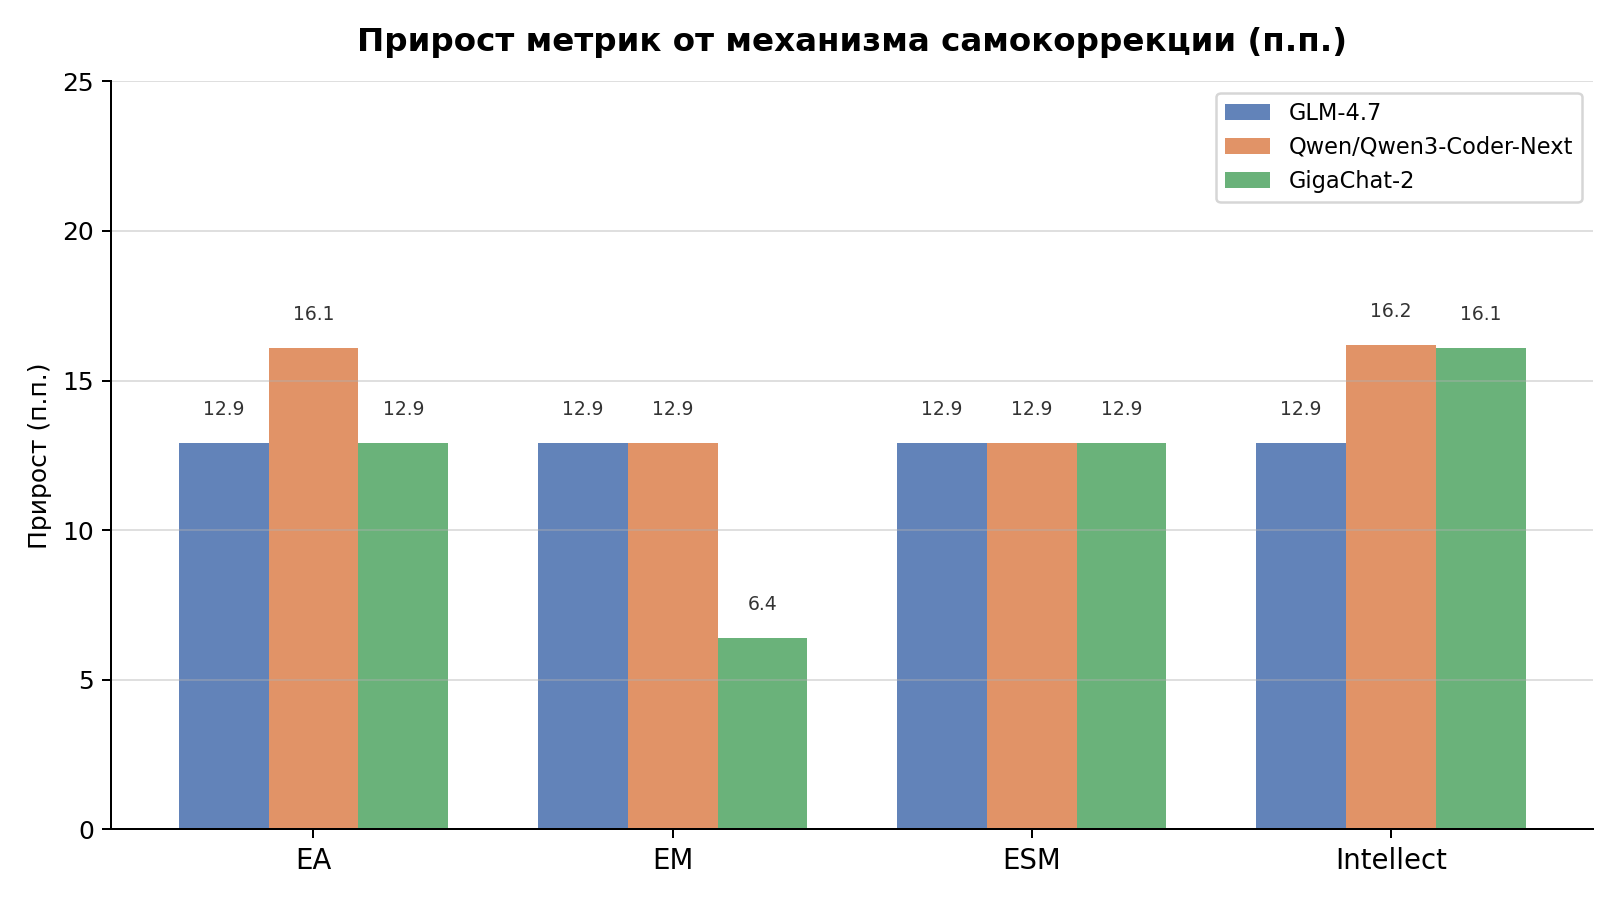
\includegraphics[width=\textwidth]{materials/llm_gain.png}
    \caption{Прирост производительности с режимом самокоррекции}
    \label{llm_gain}
\end{figure}
